\documentclass[tikz,border=7pt]{standalone}
% Shared visual language for the book's standalone vector figures.
% Keep this file compatible with the TeX Live version used by LyX.
\usepackage{amsmath,amssymb}
\usepackage{array,booktabs}
\usepackage{pgfplots}
\usepackage{pgfplotstable}
\usetikzlibrary{arrows.meta,calc,positioning}
\pgfplotsset{compat=1.17}

\definecolor{BookBlue}{HTML}{0072B2}
\definecolor{BookOrange}{HTML}{D55E00}
\definecolor{BookGreen}{HTML}{009E73}
\definecolor{BookGray}{HTML}{666666}
\definecolor{BookLightGray}{HTML}{D9D9D9}

\pgfplotsset{
  book axis/.style={
    axis line style={black!75,line width=0.55pt},
    tick style={black!75,line width=0.45pt},
    tick label style={font=\small},
    label style={font=\small},
    legend style={
      font=\small,
      draw=none,
      fill=none,
      cells={anchor=west},
    },
    grid style={BookLightGray,line width=0.35pt},
    major grid style={BookLightGray,line width=0.35pt},
  },
}

\begin{document}
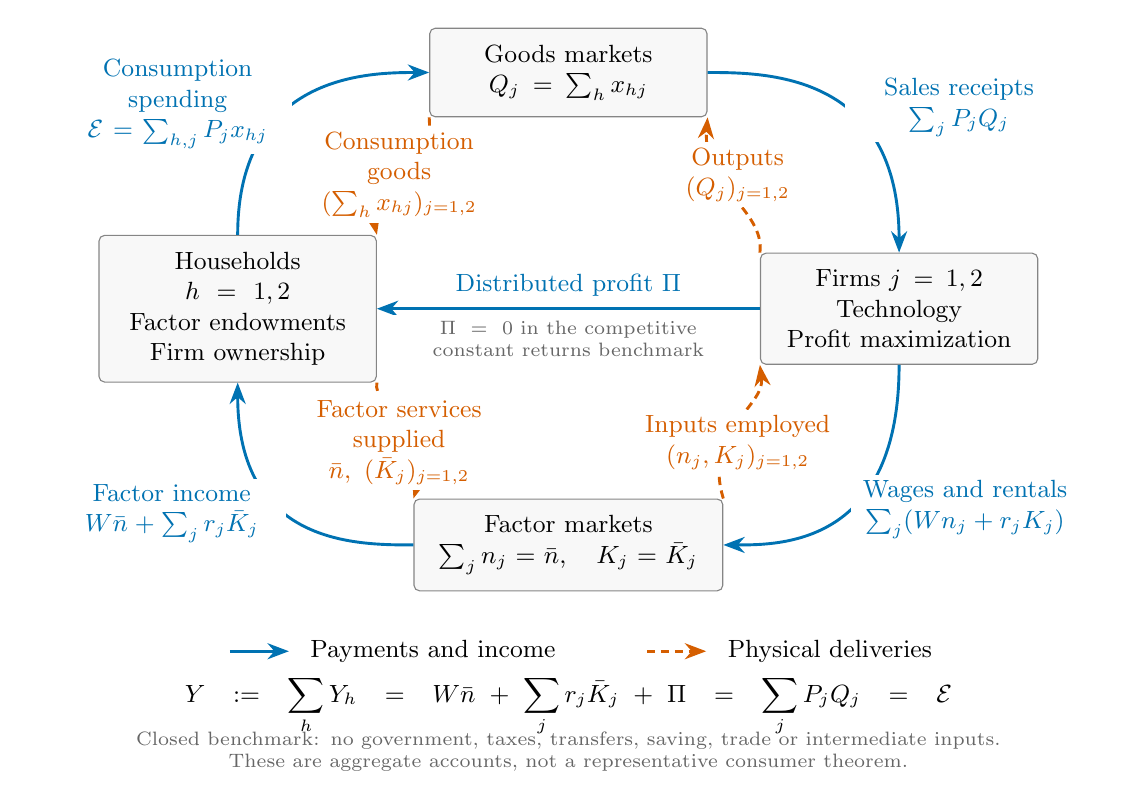
\begin{tikzpicture}[
  >=Stealth,font=\small,
  account/.style={draw=BookGray!80,rounded corners=2pt,fill=BookLightGray!18,
    minimum height=1.05cm,text width=3.1cm,align=center,inner sep=6pt},
  money/.style={->,BookBlue,line width=1.05pt},
  real/.style={->,BookOrange,line width=1.05pt,densely dashed},
  payment label/.style={text=BookBlue,align=center,font=\small,fill=white,
    inner sep=2pt,text width=2.75cm},
  real label/.style={text=BookOrange,align=center,font=\small,fill=white,
    inner sep=2pt,text width=2.55cm}
]
  \node[account] (H) at (-4.2,0)
    {Households\\$h=1,2$\\\mbox{Factor endowments}\\Firm ownership};
  \node[account] (G) at (0,3)
    {Goods markets\\$Q_j=\sum_h x_{hj}$};
  \node[account] (F) at (4.2,0)
    {Firms $j=1,2$\\Technology\\\mbox{Profit maximization}};
  \node[account,text width=3.5cm] (L) at (0,-3)
    {Factor markets\\$\sum_j n_j=\bar n,\quad K_j=\bar K_j$};

  % Money follows the outer circuit. Every label is a nominal value.
  \draw[money] (H.north) .. controls (-4.2,3) and (-2.5,3) .. (G.west)
    node[pos=.42,left,payment label] {Consumption spending\\$\mathcal E=\sum_{h,j}P_jx_{hj}$};
  \draw[money] (G.east) .. controls (2.5,3) and (4.2,3) .. (F.north)
    node[pos=.58,right,payment label] {Sales receipts\\$\sum_j P_jQ_j$};
  \draw[money] (F.south) .. controls (4.2,-3) and (2.7,-3) .. (L.east)
    node[pos=.42,right,payment label] {Wages and rentals\\$\sum_j(Wn_j+r_jK_j)$};
  \draw[money] (L.west) .. controls (-2.7,-3) and (-4.2,-3) .. (H.south)
    node[pos=.58,left,payment label] {Factor income\\$W\bar n+\sum_jr_j\bar K_j$};

  % Physical deliveries go in the opposite direction. Quantities of different
  % goods or factors are listed separately, not added as if they shared units.
  \draw[real] (G.south west) .. controls (-1.7,1.55) and (-2.5,1.25) .. (H.north east);
  \draw[real] (F.north west) .. controls (2.5,1.25) and (1.7,1.55) .. (G.south east);
  \draw[real] (H.south east) .. controls (-2.5,-1.25) and (-1.7,-1.55) .. (L.north west);
  \draw[real] (L.north east) .. controls (1.7,-1.55) and (2.5,-1.25) .. (F.south west);
  \node[real label] at (-2.15,1.7)
    {Consumption goods\\$(\sum_hx_{hj})_{j=1,2}$};
  \node[real label] at (2.15,1.7)
    {Outputs\\$(Q_j)_{j=1,2}$};
  \node[real label] at (-2.15,-1.7)
    {Factor services\\supplied\\$\bar n,\ (\bar K_j)_{j=1,2}$};
  \node[real label] at (2.15,-1.7)
    {Inputs employed\\$(n_j,K_j)_{j=1,2}$};

  % Dividends are not physical output or a second factor payment. In the
  % chapter's competitive constant returns CES benchmark this flow is zero.
  \draw[money] (F.west)--(H.east)
    node[midway,above=2pt,text=BookBlue,fill=white,inner sep=2pt]
      {Distributed profit $\Pi$};
  \node[font=\scriptsize,text=BookGray,fill=white,inner sep=2pt,
    align=center,text width=4.7cm] at (0,-.38)
    {$\Pi=0$ in the competitive\\constant returns benchmark};

  \draw[money] (-4.3,-4.35)--(-3.55,-4.35);
  \node[anchor=west] at (-3.4,-4.35) {Payments and income};
  \draw[real] (1,-4.35)--(1.75,-4.35);
  \node[anchor=west] at (1.9,-4.35) {Physical deliveries};

  \node[align=center,text width=13.5cm,font=\small] at (0,-5.05)
    {$\displaystyle Y:=\sum_hY_h=W\bar n+\sum_jr_j\bar K_j+\Pi
       =\sum_jP_jQ_j=\mathcal E$};
  \node[align=center,text width=13.5cm,font=\scriptsize,text=BookGray] at (0,-5.62)
    {Closed benchmark: no government, taxes, transfers, saving, trade or intermediate inputs.\\
     These are aggregate accounts, not a representative consumer theorem.};
\end{tikzpicture}
\end{document}
